\documentclass{beamer}
%%%%%% UNOFFICIAL ICL BEAMER TEMPLATE V.0.1 %%%%%%
% This is a basic LaTeX Beamer template that I customised to have the logo of ICL and a background picture. Mind that this is NOT an official ICL template but it may still be useful for informal presentations.
% The official ICL graphical identity resources can be found here: http://www3.imperial.ac.uk/graphicidentity
% Please drop me an e-mail or comment via Twitter @AJunyentFerre if you found this was useful or have any suggestion to improve it.
%%%%%%

\usepackage[spanish]{babel}
\usepackage[utf8]{inputenc}
\usepackage{stmaryrd}
\usepackage[T1]{fontenc}
\usepackage{lmodern}
\usepackage{algorithm2e}
%%%%%% THE FOLLOWING FILE CONTAINS THE STYLE DEFINITIONS %%%%%%
\usepackage[utf8]{inputenc}

\definecolor{gris}{rgb}{0.92,0.92,0.92}
\definecolor{blau-upc}{rgb}{.192,.365,.506}

\setbeamercolor{titlelike}{fg=blau-upc}
% \setbeamercolor{barra}{bg=white,fg=white}
\setbeamercolor{capcalera}{bg=blau-upc,fg=white}
\setbeamercolor{section in toc}{fg=blau-upc}
\setbeamertemplate{sections/subsections in toc}[circle]
\setbeamertemplate{itemize items}[circle]
\setbeamercolor{item}{fg=blau-upc}
\setbeamertemplate{blocks}[rounded][shadow=true]
\setbeamercolor*{block body}{bg=gris}
\setbeamerfont{block body}{size=\footnotesize}
\setbeamercolor*{block title}{parent=structure,bg=blau-upc,fg=white}

\setbeamersize{text margin left=12mm,text margin right=12mm}
\setbeamertemplate{navigation symbols}{}

\defbeamertemplate*{headline}{infolines theme}
{
	\begin{beamercolorbox}[wd=\paperwidth,ht=9.5mm,right]{white}%
		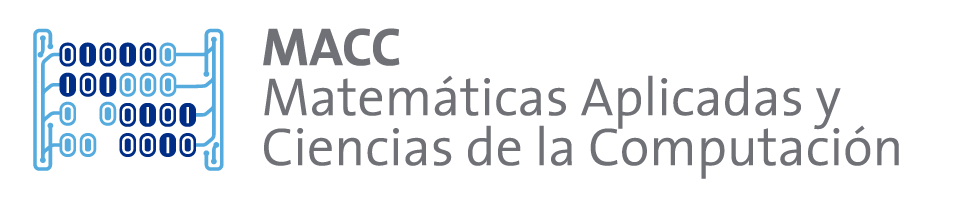
\includegraphics[height=8mm]{./logotips/macc_logo.png}\hspace*{1mm}\vskip0.2ex
	\end{beamercolorbox}
% 	\begin{beamercolorbox}[wd=\paperwidth,ht=0.5mm,left]{barra}%
% 		\hspace*{1mm}
% 	\end{beamercolorbox}
}

\setbeamertemplate{footline}
{
	\hbox{
	\begin{beamercolorbox}[wd=0.1\paperwidth,ht=10mm,left]{}
% 		\hspace*{1ex}\includegraphics[height=8mm]{./logotips/imperiallogo.pdf}\vskip 2ex
	\end{beamercolorbox}
	\begin{beamercolorbox}[wd=0.8\paperwidth,ht=3ex,center]{}
		\hspace*{4ex}\insertsection\vskip 4ex
	\end{beamercolorbox}
	\begin{beamercolorbox}[wd=0.1\paperwidth,ht=3ex,right]{}
		\insertpagenumber\hspace*{6ex}\vskip 4ex
	\end{beamercolorbox}
	}
}

\setbeamertemplate{title page}
{
	\vbox{}
	\vfill
	\begin{centering}
		{\usebeamerfont{title}\usebeamercolor[fg]{title}\inserttitle}
		\vskip0.2em
		{\usebeamerfont{subtitle}\usebeamercolor[fg]{subtitle}\insertsubtitle}
		\vskip2em\par
		\small\insertauthor\par
		\vskip0.7em\par
		\tiny\insertdate\vskip1em\par
	\end{centering}
% 	\vfill
}

\usebackgroundtemplate{\put(-10,-260){
\includegraphics[width=2.5cm]{./logotips/rosario.png}}} 
%%%%%%

%%%%%% TITLE, AUTHOR, DATE DEFINITIONS %%%%%%
\title{Implementación de la clase \texttt{Graph} en C++}
\subtitle{{\it Junto a algunos algoritmos conocidos en la teoría de grafos no dirigidos.}}
\author{Víctor Samuel Pérez Díaz\\ Juan Esteban Murcia Nieto}
\date{21 Mayo 2019}
%%%%%%

\begin{document}

\frame{\titlepage} 

\frame{\frametitle{Esquema de presentación}\tableofcontents}

\section{Introducción}

\frame{\frametitle{Contextualización}
	
	\begin{columns}
		\column{0.9\textwidth}
			\begin{itemize}
			
			\item Nuestro \textbf{objetivo} es desarrollar una estructura de datos que nos permita implementar los algoritmos clásicos de la teoría de grafos no dirigidos.
			
			\item El lenguaje de programación empleado fue \texttt{C++} debido a su eficiencia y gran versatilidad.
			
			\item Nuestro código consta de tres partes:
			
			\begin{itemize}
				\item \textbf{Interfaz} (\texttt{.hpp})
				
				\item \textbf{Implementación} (\texttt{.cpp})
				
				\item \textbf{Programa ejemplo} (\texttt{.cpp})
			\end{itemize}
		
		
			\end{itemize}
		
		\column{0.4\textwidth}
		
		
\includegraphics[scale=0.4]{./logotips/c++.png}
			

	\end{columns}
	
}

\section{Resumen}
\frame{\frametitle{Conceptos preliminares}
	
	La raiz de toda nuestra implementación es la clase \texttt{Graph}, la cual tiene como único parámetro la matriz de adyacencia (\texttt{matrix}) de un grafo $G$. 
	
	Esta está definida como: 
	\begin{block}{Matriz de adyacencia}
		{\tiny
		 \[A(G): a_{ij} = \begin{cases} 
		$1 (Por arista)$ & ,v_i \leftrightarrow v_j, i \not = j\\
		0 & ,v_i \not\leftrightarrow v_j, i \not = j \\
		$2 (Por arista)$ & ,v_i \leftrightarrow v_j, i=j
		\end{cases}
		\]
		}
	\end{block}
}

\frame{\frametitle{Conceptos preliminares}
	
	Para lo anterior, se usó la clase \texttt{vector} de librería estándar de \texttt{C++}, la cual usamos para crear un vector de vectores, que nos serviría para representar la matriz.
}

\frame{\frametitle{Conceptos preliminares}
	
	Los \textbf{métodos} desarrollados fueron:
	\begin{block}{Métodos de la clase \texttt{Graph}}
	{\tiny
		\begin{itemize}
			\item \texttt{Graph} \textit{constructor y sus derivados.}
			\item \texttt{uncolored\_vertex}
			\item \texttt{colored\_vertex}
			\item \texttt{colored\_neighbor}
			\item \texttt{uv\_path}
			\item \texttt{grade}
			\item \texttt{empty}
			\item \texttt{order}
			\item \texttt{size}
			\item \texttt{max\_grade}
			\item \texttt{min\_grade}
		\end{itemize}
	}
	\end{block}
}

\frame{\frametitle{Conceptos preliminares}
	
	Los \textbf{métodos} desarrollados fueron:
	\begin{block}{Métodos de la clase \texttt{Graph}}
		{\tiny
			\begin{itemize}
				\item \texttt{remove\_node}
				\item \texttt{remove\_edge}
				\item \texttt{add\_node}
				\item \texttt{add\_edge}
				\item \texttt{clear}
				\item \texttt{print\_matrix}	
				\item \texttt{find\_path}
				\item \texttt{color\_graph}
				\item \texttt{breadth\_search}
				\item \texttt{depth\_search}
				\item \texttt{shortest\_uv\_path}
			\end{itemize}
		}
	\end{block}
}

\section{Funcionalidad}

\frame{\frametitle{Funcionalidad}
	
	La clase \texttt{Graph} está basada en la matriz de adyacencia de un grafo no dirigido, esta siendo su único parámetro.
	
	Un primer acercamiento fue creando dos estructuras \texttt{nodos (V)} y \texttt{aristas (E)}, pero resultaba un tanto conflictiva en la manipulación de la memoria.
	
	La implementación representando el grafo mediante su matriz resultaba mucho más \textbf{práctica}.
}

\frame{\frametitle{Constructor \texttt{Graph}}
	
	Se desarrollaron varias versiones del constructor:
	\begin{block}{Constructores de la clase \texttt{Graph}}
	{\tiny
		\begin{itemize}
			\item \texttt{Graph()}: Constructor vacío, un grafo sin nodos ni aristas.
			\item \texttt{Graph(Graph)}: Constructor copia.
			\item \texttt{Graph(A\_matrix)}: Construye un grafo con una matriz de adyacencia específica.
			\item \texttt{Graph(filename)}: Construye un grafo con una matriz de adyacencia específica contenida en un archivo \texttt{.txt}.
		\end{itemize}
	}
	\end{block}
	

}

\frame{\frametitle{Funciones Privadas}
	
	La clase cuenta con varias funciones las cuales no tienen un uso especial para el usuario, pero son cruciales para la buen funcionamiento de ciertos algoritmos, razón por la cual fueron definidas como privadas:
	\begin{block}{Funciones privadas}
		{\tiny
			\begin{itemize}
			\item \texttt{$uncolored\_vertex$}: Dada una colaroción para el grafo, esta función determina si el nodo tiene o no color
			\item \texttt{$colored\_neighbor$}: Dada una coloración para el grafo, esta función determina si un nodo tiiene algún vecino con un color específico
			\item \texttt{$uv\_path$}: Función que determina si hay un uv-camino en el grafo
			\end{itemize}
		}
	\end{block}
	
	
}

\frame{\frametitle{Funciones públicas}
	
	La clase le otorga al usuario diversas funciones con objetivos generales, cuyo objetivo es conocer y manipular el grafo que está trabajando.
	\begin{block}{Funciones Públicas}
		{\tiny
			\begin{itemize}
				\item \texttt{grade}: Retorna el grado de un nodo específico
				\item \texttt{empty}: Determina si el grafo está vacío
				\item \texttt{order}: Retorna la cantidad de nodos del grafo
				\item \texttt{size}: Retorna la cantidad de aristas del grafo
				\item \texttt{max\_grade}: Retorna el grado máximo del grafo, $\Delta$(G)
				\item \texttt{min\_grade}: Retorna el grado mínimo del grafo, $\delta$(G)
				\item \texttt{remove\_node}: Elimina un nodo específico del grafo y todas sus aristas adyacentes
				\item \texttt{remove \_edge}: Elimina una arista específica del grafo
				\item \texttt{add\_node}: Añade un nodo al grafo, sin ninguna arista
				\item \texttt{add\_edge}: Añade una arista entre 2 nodos específicos
				\item \texttt{clear}: Elimina todos los nodos y todas las aristas del grafo
				\item \texttt{print\_matrix}: Imprime la matriz de adyacenciadel grafo
			\end{itemize}
		}
	\end{block}
	
	
}

\section{Algoritmos}
\frame{
	\vbox{}
	% 	\vfill
	\begin{centering}
		{\LARGE \usebeamercolor[fg]{title} Algoritmos}
		\par
	\end{centering}
}
\frame{\frametitle{\texttt{find\_path}}
\begin{algorithm}[H]
	\caption{Eulerian path}
	\KwOut{An Eulerian path}
	Initialization:\\
	path,stk = empty\\
	start, odd = 0\\
	\For{i in 1:n(G)} {
		\If{grade(i) is odd} {
			odd += 1\\
			start = i\\
		}
	}
	\If{odd > 2}{
		return empty\\
	}
	cur = start\\
\end{algorithm}

}

\frame{
	\begin{algorithm}[H]
		\While{stk not empty or garde(cur) > 0} {
			\If{grade(cur) == 0} {
				path.push(cur)\\
				cur = stk.top\\
				stk.pop\\
			}
		\Else {
			\For{i=1:n(G)}{
				\If{cur$\leftrightarrow$i}{
					stk.push(cur)\\
					\texttt{remove\_edge}(cur,i)\\
					cur = i\\
					break\\
				}
			}
		}
	}
	return path\\
	\end{algorithm}
}

\frame{\frametitle{\texttt{color\_graph}}
	\begin{algorithm}[H]
		\caption{greedy coloring}
		\KwOut{A colored graph}
		out= (n,0)\\
		clr = 1\\
		\While{\texttt{Unolored\_vertex}} {
			\For{i=1:n(G)}{
				\If{i has no color and not \texttt{colored\_neighbor}} {
					out[i] = clr	\\
				}
			}
		clr += 1
		}
	return out
	\end{algorithm}
}

\frame{\frametitle{\texttt{shrtest\_uv\_path}}
	\begin{algorithm}[H]
		\caption{Dijkstras Algorithm}
		\KwOut{sortest uv path}
		values[i] = 0 if i=u, $\infty$ if not\\
		Tm = nodes\\
		path[i] = $\infty$\\
		\While{v in Tm}{
			vertex = i in Tm: values[i] is minimum\\
			erase i from Tm\\
			\For{i in nodes}{
				\If{vertex$\leftrightarrow$i and values[vertex]+1 < values[i]} {
					values[i] = values[vertex]+1\\
					path[i] = vertex
				}
			}
		}
	\end{algorithm}
}

\frame{
	\begin{algorithm}[H]
		\If{path[v] = $\infty$}{
			return empty
		}
		push u to out\\
		cur = v\\
		\While{cur != u}{
			insert cur in the $2^{nd}$ position of out\\
			cur = path[cur]\\
		}
	return out
	\end{algorithm}
}

\frame{
	También se implementaron algoritmos ya conocidos como:
	
	\begin{itemize}
			\item \texttt{breadth\_search}
			\item \texttt{depth\_search}
	\end{itemize}
}

\section{Ejemplos}
\frame{\frametitle{Ejemplo}
	Eejmplificaremos todos los algoritmos previamente explicados con el siguiente grafo:\\
	\begin{figure}
	\label{El grafeno}
	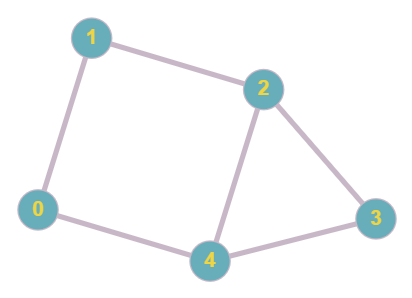
\includegraphics[scale=0.4]{grafo1.png}
	\caption{Grafo}
	\end{figure}
}

\begin{frame}[allowframebreaks]
\begin{thebibliography}{10}
	\bibitem{first}
	\alert{Douglas B. West}
	\newblock  {Introduction to graph theory.}
	\newblock {\em  New Delhi: Prentice-
		Hall of India Private Limited. (2005)}.
	
	\bibitem{secl d}
	\alert{Geeks for geeks}
	\newblock {A computer    science    portal    for    geeks.    (n.d.).    Retrieved    from
		https://www.geeksforgeeks.org/}
	\newblock {\em Algorithms in graph theory}.
\end{thebibliography}
\end{frame}

\section*{ }
\frame{
 	\vbox{}
% 	\vfill
	\begin{centering}
	{\LARGE \usebeamercolor[fg]{title} ¡Gracias!}
	\par
	\end{centering}
}

\end{document}